\begin{vd}[Xoắn dây]
    Một vòng dây được uốn thành hình dạng như trong hình dưới. Vòng dây được đặt trong từ trường đều và tăng dần với $\dfrac{\mathrm{d}B}{\mathrm{d}t}=2,34\dv{T/s}$. Cho biết diện tích các phần như sau $A=4,23\dv{m^2}$, $B=2,74\dv{m^2}$ và $C=0,34\dv{m^2}$ (phần diện tích $B$ không bao gồm $C$). Tính độ lớn suất điện động cảm ứng trong dây.
    %chèn hình
    \begin{center}

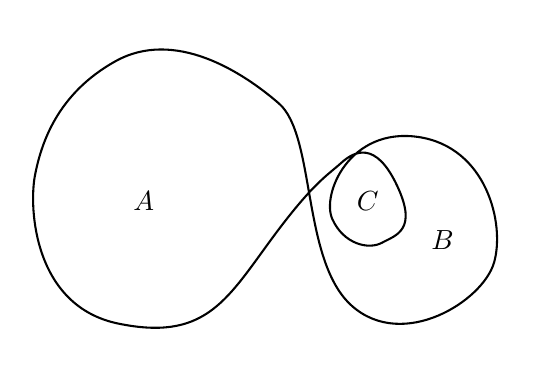
\begin{tikzpicture}[x=0.75pt,y=0.75pt,yscale=-1,xscale=1]
%uncomment if require: \path (0,162); %set diagram left start at 0, and has height of 162

%Shape: Polygon Curved [id:ds4706242055483567] 
\draw   (397.45,57.78) .. controls (364.48,52.98) and (350.69,85.35) .. (356.09,97.34) .. controls (361.48,109.33) and (373.47,112.33) .. (380.06,108.73) .. controls (386.66,105.13) and (397.45,102.74) .. (387.26,81.16) .. controls (377.07,59.58) and (366.88,64.37) .. (360.28,70.37) .. controls (353.69,76.36) and (346.49,79.96) .. (325.51,108.73) .. controls (304.53,137.5) and (293.74,156.09) .. (252.98,147.7) .. controls (212.22,139.3) and (209.82,91.95) .. (212.82,76.36) .. controls (215.82,60.78) and (223.61,36.8) .. (251.78,21.21) .. controls (279.96,5.63) and (312.33,26.01) .. (330.31,41.59) .. controls (348.29,57.18) and (341.1,117.72) .. (365.68,139.3) .. controls (390.25,160.88) and (428.62,136.91) .. (434.01,118.32) .. controls (439.41,99.74) and (430.42,62.57) .. (397.45,57.78) -- cycle ;

% Text Node
\draw (258.76,82.4) node [anchor=north west][inner sep=0.75pt]    {$A$};
% Text Node
\draw (402.33,101.24) node [anchor=north west][inner sep=0.75pt]    {$B$};
% Text Node
\draw (366.46,82.66) node [anchor=north west][inner sep=0.75pt]    {$C$};


\end{tikzpicture}

    \end{center}
    \end{vd}

\begin{vd}[Đứt cầu ch...]%câu 13
%USAPhO 2010
Ba phần của bài này có thể trả lời độc lập.
\begin{enumerate}[1.]
    \item Có hai sợi dây dẫn điện dài, song song với nhau, một đầu của mỗi dây được nối với một điện trở $R=0,25~ \mathrm{\Omega}$ và một cầu chì sẽ đứt tức thì nếu có dòng điện $5~ \mathrm{A}$ chạy qua nó. Đầu còn lại của chúng được để tự do. Một thanh dẫn khối lượng $m$ trượt tự do dọc theo dây dưới tác dụng của trọng lực. Hai dây cách nhau $30~ \mathrm{cm}$, thanh bắt đầu chuyển động từ vị trí cách điện trở và cầu chì $10~\mathrm{cm}$. Cả hệ được đặt trong từ trường đều, không đổi $B=1,2\ \mathrm{T}$ như hình vẽ. Điện trở của dây dẫn và của thanh không đáng kể. Khi thanh được thả, nó rơi dưới tác dụng của trọng lực nhưng luôn tiếp xúc với hai dây dẫn.
    \begin{center}
        

\tikzset{every picture/.style={line width=0.75pt}} %set default line width to 0.75pt        

\begin{tikzpicture}[x=0.75pt,y=0.75pt,yscale=-1,xscale=1]
%uncomment if require: \path (0,418); %set diagram left start at 0, and has height of 418

%Straight Lines [id:da17090281026704623] 
\draw    (121,70) -- (121,328) ;
%Straight Lines [id:da5878220563298939] 
\draw    (367,70) -- (367,328) ;
%Shape: Rectangle [id:dp9840410277040863] 
\draw  [fill={rgb, 255:red, 255; green, 255; blue, 255 }  ,fill opacity=1 ] (94,203) -- (397,203) -- (397,229) -- (94,229) -- cycle ;
%Shape: Resistor [id:dp49773719674779127] 
\draw   (121,70) -- (135.4,70) -- (138.6,50) -- (145,90) -- (151.4,50) -- (157.8,90) -- (164.2,50) -- (170.6,90) -- (177,50) -- (183.4,90) -- (186.6,70) -- (201,70) ;
%Straight Lines [id:da33406599682703697] 
\draw    (201,70) -- (230,70) ;
%Shape: Rectangle [id:dp3926228662226221] 
\draw  [fill={rgb, 255:red, 155; green, 155; blue, 155 }  ,fill opacity=1 ] (231,63) -- (308,63) -- (308,77) -- (231,77) -- cycle ;
%Straight Lines [id:da6386859233763178] 
\draw    (309,70) -- (367,70) ;

% Text Node
\draw (134,96.4) node [anchor=north west][inner sep=0.75pt]    {$\text{Điện trở}$};
% Text Node
\draw (244,95.4) node [anchor=north west][inner sep=0.75pt]    {$\text{Cầu chì}$};
% Text Node
\draw (196,170.4) node [anchor=north west][inner sep=0.75pt]    {$\text{Thanh trượt}$};
% Text Node
\draw (122,244.4) node [anchor=north west][inner sep=0.75pt]    {Từ trường có hướng đi vào trang giấy };


\end{tikzpicture}

    \end{center}
    \begin{enumerate}[a)]
        \item Khối lượng của thanh dẫn nhỏ nhất bằng bao nhiêu để làm đứt cầu chì?
        \item Vận tốc của thanh là bao nhiêu sau khi cầu chì bị đứt?
    \end{enumerate}
    \item Một cầu chì được cấu tạo bởi một dây dẫn hình trụ chiều dài $L$ với bán kính là $r\ll L$. Điện trở suất (không phải điện trở!) của cầu chì là $\rho_f$ nhỏ. Giả sử rằng một dòng điện đều $I$ chạy qua cầu chì. Biểu diễn các kết quả của bạn theo $L, r, \rho_f, I$ và các hằng số cơ bản.
    \begin{enumerate}[a)]
        \item Hãy tìm độ lớn và hướng của điện trường trên bề mặt dây cầu chì?
        \item Hãy tìm độ lớn và hướng của từ trường trên bề mặt dây cầu chì?
        \item Vector Poynting $\overrightarrow{S}$ là một đại lượng đo tốc độ năng lượng điện từ qua một đơn vị diện tích, vector cho biết hướng của dòng năng lượng. Với $\ot{S}=\dfrac{1}{\mu_0}\ot{E}\times\ot{B}$, với $\mu_0$ là độ từ thẩm chân không, $\ot{E}$ và $\ot{B}$ lần lượt là vector điện trường và từ trường, hãy tìm độ lớn và hướng của vector Poynting liên quan với dòng điện trong cầu chì.
    \end{enumerate}
    \item Cầu chì sẽ đứt khi nó đạt tới điểm nóng chảy. Chúng ta biết từ vật lí hiện đại rằng một vật thể nóng sẽ bức xạ năng lượng (xấp xỉ) theo định luật vật đen: $P=\sigma A T^4$, trong đó $T$ là nhiệt độ theo nhiệt giai Kelvin, $A$ là diện tích bề mặt, và $\sigma$ là hằng số Stefan-Boltzmann. Nếu $T_f=500\ \mathrm{K}$ là điểm nóng chảy của kim loại làm cầu chì, với điện trở suất $\rho_f=120\ \mathrm{n\Omega\cdot m}$, và $I_f=5\ \mathrm{A}$ là cường độ dòng điện mong muốn khi cầu chì đứt, bán kính $r$ của cầu chì bằng bao nhiêu?
    \end{enumerate}
\end{vd}

\begin{vd}[Dây dẫn dài]
Giả sử rằng chúng ta có một thiết bị điện được nối vào nguồn $U_0 = 120$V một chiều thông qua một dây dẫn dài. Vì các phần tử của thiết bị điện gần với nhau nên ta có một sơ đồ mạch tương đương như hình vẽ.
   \begin{center}


\tikzset{every picture/.style={line width=0.75pt}} %set default line width to 0.75pt        

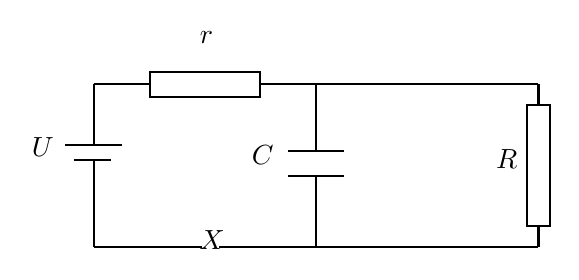
\begin{tikzpicture}[x=0.75pt,y=0.75pt,yscale=-1,xscale=1]
%uncomment if require: \path (0,300); %set diagram left start at 0, and has height of 300

%Straight Lines [id:da992635552977859] 
\draw    (159.43,99.05) -- (266.58,99.05) ;
%Shape: Rectangle [id:dp40515807470760334] 
\draw  [fill={rgb, 255:red, 255; green, 255; blue, 255 }  ,fill opacity=1 ] (186.38,92.98) -- (239.64,92.98) -- (239.64,105.13) -- (186.38,105.13) -- cycle ;
%Straight Lines [id:da9013646240831978] 
\draw    (266.58,131.38) -- (266.58,99.05) ;
%Straight Lines [id:da843756955596408] 
\draw    (266.58,99.05) -- (373.73,99.05) ;
%Straight Lines [id:da6880281635624372] 
\draw    (373.73,177.42) -- (373.73,99.05) ;
%Straight Lines [id:da10033565086863971] 
\draw    (266.58,177.42) -- (373.73,177.42) ;
%Straight Lines [id:da7517210738689919] 
\draw    (219.88,177.42) -- (266.58,177.42) ;
%Straight Lines [id:da6294900742240948] 
\draw    (159.43,128.44) -- (159.43,99.05) ;
%Straight Lines [id:da7676124152868049] 
\draw    (159.43,177.42) -- (159.43,135.3) ;
%Straight Lines [id:da9227393314302665] 
\draw    (145.83,128.44) -- (173.04,128.44) ;
%Straight Lines [id:da4284739815829446] 
\draw    (149.99,135.3) -- (167.79,135.3) ;
%Straight Lines [id:da08072848111989406] 
\draw    (266.58,177.42) -- (266.58,143.13) ;
%Straight Lines [id:da44210756207608326] 
\draw    (252.98,131.38) -- (280.19,131.38) ;
%Straight Lines [id:da8980247380162103] 
\draw    (252.98,143.13) -- (280.19,143.13) ;
%Shape: Rectangle [id:dp25862548825541065] 
\draw  [fill={rgb, 255:red, 255; green, 255; blue, 255 }  ,fill opacity=1 ] (379.3,109.19) -- (379.3,167.28) -- (368.16,167.28) -- (368.16,109.19) -- cycle ;
%Straight Lines [id:da8646847580277894] 
\draw    (159.43,177.42) -- (211.8,177.42) ;


% Text Node
\draw (209.02,168.25) node [anchor=north west][inner sep=0.75pt]    {$X$};
% Text Node
\draw (128.13,123.19) node [anchor=north west][inner sep=0.75pt]    {$U$};
% Text Node
\draw (234.17,127.11) node [anchor=north west][inner sep=0.75pt]    {$C$};
% Text Node
\draw (209.07,72.25) node [anchor=north west][inner sep=0.75pt]    {$r$};
% Text Node
\draw (351.82,129.07) node [anchor=north west][inner sep=0.75pt]    {$R$};


\end{tikzpicture}
\end{center}
Điện trở $R$ chính là thiết bị điện, điện trở $r \ll R$ đặc trưng cho điện trở của dây dẫn và tụ điện có điện dung $C=420\,\mathrm{nF}$ đặc trưng cho trở kháng của dây. Điểm được đánh dấu $X$ trên mạch là một điểm nối tiếp xúc kém, do đó nó sẽ đóng mở mạch theo các chu kì. Mỗi nửa chu kì đóng và mở đều kéo dài $0,001~\mathrm{s}$. Tìm công suất mà nguồn điện cung cấp cho thiết bị điện sau một thời gian rất dài mạch được đóng. Cho rằng nếu điểm tiếp xúc là ổn định (không bị đóng mở theo chu kì) thì công suất cung cấp bởi nguồn sẽ là $P_0 = 30~\mathrm{W}$.
\end{vd}